\documentclass[11pt,a4paper]{article}
\usepackage[margin=1in]{geometry}
\usepackage{amsmath,amssymb}
\usepackage{graphicx}
\usepackage{enumitem}
\usepackage{tcolorbox}
\usepackage{array}
\usepackage{multirow}
\usepackage{tikz}
\usetikzlibrary{positioning,arrows.meta,shapes}

% Custom commands
\newcommand{\highlight}[1]{\textbf{#1}}

% Box for exercises
\newtcolorbox{exercise}[1][]{
    colback=blue!5!white,
    colframe=blue!75!black,
    title=#1,
    fonttitle=\bfseries
}

\newtcolorbox{hint}[1][]{
    colback=yellow!10!white,
    colframe=orange!75!black,
    title=Hint,
    fonttitle=\bfseries
}

\newtcolorbox{concept}[1][]{
    colback=green!5!white,
    colframe=green!75!black,
    title=#1,
    fonttitle=\bfseries
}

\title{\textbf{Week 2: Word2Vec Deep Dive}\\
\large Understanding CBOW, Skip-gram, and Negative Sampling\\
\large Pre-Lab Exercise (No Programming Required)}
\author{NLP Course 2025 - Student Version}
\date{}

\begin{document}
\maketitle

\noindent\textbf{Time:} 30-40 minutes\\
\textbf{Objective:} Master the core mechanisms of Word2Vec by understanding what goes in (context), how it's processed (method), and what comes out (prediction).

\section*{Part 1: Understanding Context Windows (10 minutes)}

\begin{exercise}[Context Window Discovery]
Consider this sentence: \textbf{``The quick brown fox jumps over the lazy dog''}

With a context window size of 2 (two words on each side), let's analyze the word ``fox'':

\textbf{Questions:}
\begin{enumerate}
    \item Circle the context words for ``fox'' (window size = 2):
    
    \texttt{The \quad quick \quad brown \quad \fbox{fox} \quad jumps \quad over \quad the \quad lazy \quad dog}
    
    \item What are the context words? \rule{5cm}{0.4pt}
    
    \item For the word ``jumps'', what would be the context words (window size = 2)?
    
    Context words: \rule{5cm}{0.4pt}
    
    \item \textbf{Key Question:} In a context window approach:
    \begin{itemize}
        \item What is the \textbf{CONTEXT}? \rule{6cm}{0.4pt}
        \item What is the \textbf{METHOD}? \rule{6cm}{0.4pt}
        \item What is the \textbf{PREDICTION}? \rule{6cm}{0.4pt}
    \end{itemize}
\end{enumerate}
\end{exercise}

\section*{Part 2: CBOW - Continuous Bag of Words (10 minutes)}

\begin{concept}[CBOW Principle]
CBOW predicts a target word given its surrounding context words. Think of it as a ``fill in the blank'' task.
\end{concept}

\begin{exercise}[CBOW in Action]
Given the sentence: ``The cat sat on the \underline{\hspace{1cm}} mat''

\textbf{Task 1: Manual CBOW}
\begin{enumerate}
    \item Context words given: [``cat'', ``sat'', ``on'', ``the'', ``mat'']
    
    What word would you predict for the blank? \rule{3cm}{0.4pt}
    
    \item Now consider: ``I love to \underline{\hspace{1cm}} pizza for dinner''
    
    Context words: [``I'', ``love'', ``to'', ``pizza'']
    
    Your prediction: \rule{3cm}{0.4pt}
\end{enumerate}

\textbf{Task 2: CBOW Analysis}
Complete the following table for CBOW:

\begin{center}
\begin{tabular}{|l|p{8cm}|}
\hline
\textbf{Aspect} & \textbf{Your Answer} \\
\hline\hline
INPUT (Context) & \rule{7cm}{0.4pt} \\
& \\
\hline
METHOD & \rule{7cm}{0.4pt} \\
(How does it work?) & \rule{7cm}{0.4pt} \\
& \\
\hline
OUTPUT/PREDICTION & \rule{7cm}{0.4pt} \\
& \\
\hline
\end{tabular}
\end{center}

\textbf{Visual Representation:} Draw arrows showing the flow:
\begin{center}
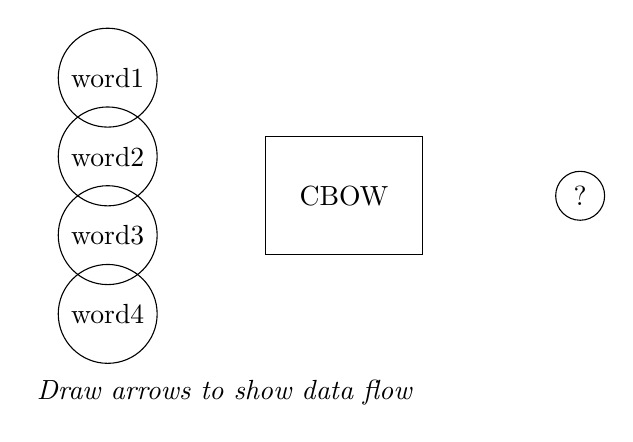
\begin{tikzpicture}
    % Input context words
    \node[draw, circle] (w1) at (0,2) {word1};
    \node[draw, circle] (w2) at (0,1) {word2};
    \node[draw, circle] (w3) at (0,0) {word3};
    \node[draw, circle] (w4) at (0,-1) {word4};
    
    % Model
    \node[draw, rectangle, minimum width=2cm, minimum height=1.5cm] (model) at (3,0.5) {CBOW};
    
    % Output
    \node[draw, circle] (out) at (6,0.5) {?};
    
    % Add your arrows here to show the flow
    \node at (1.5,-2) {\textit{Draw arrows to show data flow}};
\end{tikzpicture}
\end{center}
\end{exercise}

\section*{Part 3: Skip-gram - Predicting Context (10 minutes)}

\begin{concept}[Skip-gram Principle]
Skip-gram does the opposite of CBOW: given a center word, predict the surrounding context words.
\end{concept}

\begin{exercise}[Skip-gram in Action]
Given the center word ``\textbf{coffee}'' in: ``I drink coffee every morning''

\textbf{Task 1: Manual Skip-gram}
\begin{enumerate}
    \item What context words would you expect around ``coffee''? List 4 likely words:
    \begin{itemize}
        \item \rule{3cm}{0.4pt}
        \item \rule{3cm}{0.4pt}
        \item \rule{3cm}{0.4pt}
        \item \rule{3cm}{0.4pt}
    \end{itemize}
    
    \item Given center word ``\textbf{king}'', what context words might appear?
    \begin{itemize}
        \item \rule{3cm}{0.4pt}
        \item \rule{3cm}{0.4pt}
    \end{itemize}
\end{enumerate}

\textbf{Task 2: Skip-gram Analysis}
Complete the following table for Skip-gram:

\begin{center}
\begin{tabular}{|l|p{8cm}|}
\hline
\textbf{Aspect} & \textbf{Your Answer} \\
\hline\hline
INPUT (Context) & \rule{7cm}{0.4pt} \\
& \\
\hline
METHOD & \rule{7cm}{0.4pt} \\
(How does it work?) & \rule{7cm}{0.4pt} \\
& \\
\hline
OUTPUT/PREDICTION & \rule{7cm}{0.4pt} \\
& \\
\hline
\end{tabular}
\end{center}

\textbf{Task 3: CBOW vs Skip-gram}
\begin{enumerate}
    \item Which approach has MORE training examples from the same sentence?
    
    \rule{5cm}{0.4pt}
    
    \item Why? \vspace{1.5cm}
\end{enumerate}
\end{exercise}

\section*{Part 4: Negative Sampling - Making Training Efficient (10 minutes)}

\begin{concept}[Why Negative Sampling?]
Training Word2Vec on large vocabularies (e.g., 50,000 words) is computationally expensive. Negative sampling speeds this up by only updating a small subset of weights.
\end{concept}

\begin{exercise}[Understanding Negative Sampling]
\textbf{Task 1: Positive vs Negative Pairs}

Given the sentence: ``The dog barked loudly''

With center word ``dog'' and context word ``barked'':
\begin{enumerate}
    \item This is a \underline{\hspace{2cm}} pair (positive/negative) because \rule{4cm}{0.4pt}
    
    \item Now consider ``dog'' and ``elephant''. This is a \underline{\hspace{2cm}} pair because \rule{4cm}{0.4pt}
    
    \item Create 3 negative pairs for center word ``dog'':
    \begin{itemize}
        \item (dog, \rule{2cm}{0.4pt})
        \item (dog, \rule{2cm}{0.4pt})
        \item (dog, \rule{2cm}{0.4pt})
    \end{itemize}
\end{enumerate}

\textbf{Task 2: The Sampling Process}

Instead of updating all 50,000 word weights, negative sampling:
\begin{enumerate}
    \item Updates the positive pair: (dog, barked) → predict ``1'' (real pair)
    \item Randomly samples k negative words (e.g., k=5)
    \item Updates these negative pairs: (dog, random\_word) → predict ``0'' (fake pair)
\end{enumerate}

\textbf{Complete this table for Negative Sampling:}

\begin{center}
\begin{tabular}{|l|p{8cm}|}
\hline
\textbf{Aspect} & \textbf{Your Answer} \\
\hline\hline
INPUT (Context) & \rule{7cm}{0.4pt} \\
& \rule{7cm}{0.4pt} \\
\hline
METHOD & \rule{7cm}{0.4pt} \\
(How does it work?) & \rule{7cm}{0.4pt} \\
& \\
\hline
OUTPUT/PREDICTION & \rule{7cm}{0.4pt} \\
& \\
\hline
\end{tabular}
\end{center}

\textbf{Task 3: Efficiency Analysis}
\begin{enumerate}
    \item Without negative sampling, how many weights update for each training example?
    
    \rule{5cm}{0.4pt}
    
    \item With negative sampling (k=5), how many weights update?
    
    \rule{5cm}{0.4pt}
    
    \item What is the speedup factor for a 50,000-word vocabulary?
    
    \rule{5cm}{0.4pt}
\end{enumerate}
\end{exercise}

\begin{hint}
Negative sampling converts the problem from multi-class classification (50,000 classes) to binary classification (real vs fake pairs).
\end{hint}

\section*{Part 5: Putting It All Together (5 minutes)}

\begin{exercise}[Synthesis]
Complete this comparison table:

\begin{center}
\begin{tabular}{|l|c|c|c|}
\hline
\textbf{Aspect} & \textbf{CBOW} & \textbf{Skip-gram} & \textbf{Negative Sampling} \\
\hline\hline
\textbf{Input} & Context words & & \\
& & & \\
\hline
\textbf{Method} & Average/combine & & Binary \\
& context & & classification \\
\hline
\textbf{Output} & & Context words & \\
& & & \\
\hline
\textbf{Best for} & Frequent & & \\
& words & & \\
\hline
\textbf{Training} & Faster & & Makes both \\
\textbf{Speed} & & & faster \\
\hline
\end{tabular}
\end{center}

\textbf{Reflection Questions:}
\begin{enumerate}
    \item Why might Skip-gram work better for rare words than CBOW?
    
    \vspace{2cm}
    
    \item How does negative sampling change what the model is learning to predict?
    
    \vspace{2cm}
    
    \item If you wanted to find similar words to ``doctor'', which approach (CBOW or Skip-gram) would likely give better results? Why?
    
    \vspace{2cm}
\end{enumerate}
\end{exercise}

\vspace{1cm}
\noindent\rule{\textwidth}{0.4pt}
\begin{center}
\textit{End of Student Exercise}
\end{center}

\end{document}